\documentclass[11pt]{beamer}

\usepackage[english]{babel}
\usepackage[T1]{fontenc}
\usepackage[utf8]{inputenc}
\usepackage{mathtools}                       % matma
\usepackage{amsfonts,amsmath,amssymb,amsthm} % matma
\usepackage{listings}                        % załączanie kodu źródłowego
\usepackage{tikz}                            % rysowanie i grafy https://tikz.dev/tikz, https://centrality.mimuw.edu.pl/editor
\usepackage{pgf}
\usepackage{graphicx}
\usepackage{algorithm,algpseudocode}

\title{NetworkX Graph Visualization}
\author{Stanisław Bitner, Aleksander Wojsz}
\date{\today}

\usetheme{Warsaw}
\usecolortheme{orchid}

\setbeamertemplate{footline}[Warsaw]
\setbeamertemplate{headline}{}
\setbeamertemplate{page number in head/foot}[totalframenumber]
\setbeamertemplate{navigation symbols}{}

\usetikzlibrary{positioning,overlay-beamer-styles,graphs,fit,shapes}
\tikzset{}

\lstset{basicstyle=\ttfamily\footnotesize,keywordstyle=\color{magenta},tabsize=2,escapeinside=||,mathescape=true}

\begin{document}

\frame{\titlepage}

\begin{frame}
    \frametitle{Table of contents}
    \tableofcontents[hideallsubsections]
\end{frame}

\section{Intro}
\begin{frame}{\secname}
    \tableofcontents[currentsection,hideothersubsections,sectionstyle=hide]
\end{frame}

\subsection{Math Representation}
\begin{frame}{\subsecname}
    \begin{align*}
        G &= \left\langle V, E \right\rangle\\
        V &= \left\{ 1 \hdots 9 \right\}\\
        E &= \{\\
            &\{ 1, 2 \}, \{ 1, 3 \}, \{ 2, 4 \}, \{ 2, 5 \}, \{ 2, 6 \},\\
            &\{ 3, 5 \}, \{ 3, 6 \}, \{ 4, 7 \}, \{ 4, 8 \}, \{ 5, 7 \},\\
            &\{ 5, 8 \}, \{ 6, 7 \}, \{ 6, 8 \}, \{ 7, 9 \}, \{ 8, 9 \}\\
        \}
    \end{align*}
    
    \pause\center\Huge\textcolor{red}{TERRIBLE!!!}
\end{frame}

\subsection{Problem statement}
\begin{frame}{\subsecname}
    \begin{block}{Input}
        Graph $G = \langle V,E \rangle$
    \end{block}
    \pause
    \begin{block}{Output}
        Clear and readable drawing of $G$ (we focus on straight-line edges).
    \end{block}
    \pause
    \begin{block}{Criteria}
        \begin{itemize}
            \pause\item adjacent vertices close
            \pause\item non-adjacent vertices distant
            \pause\item short and similar in length edges
            \pause\item as few crossings as possible
            \pause\item nodes distributed evenly
            \pause\item clusters together
        \end{itemize}
    \end{block}
\end{frame}

\subsection{Hand Drawing}
\begin{frame}{\subsecname}
    \begin{figure}
        \centering
        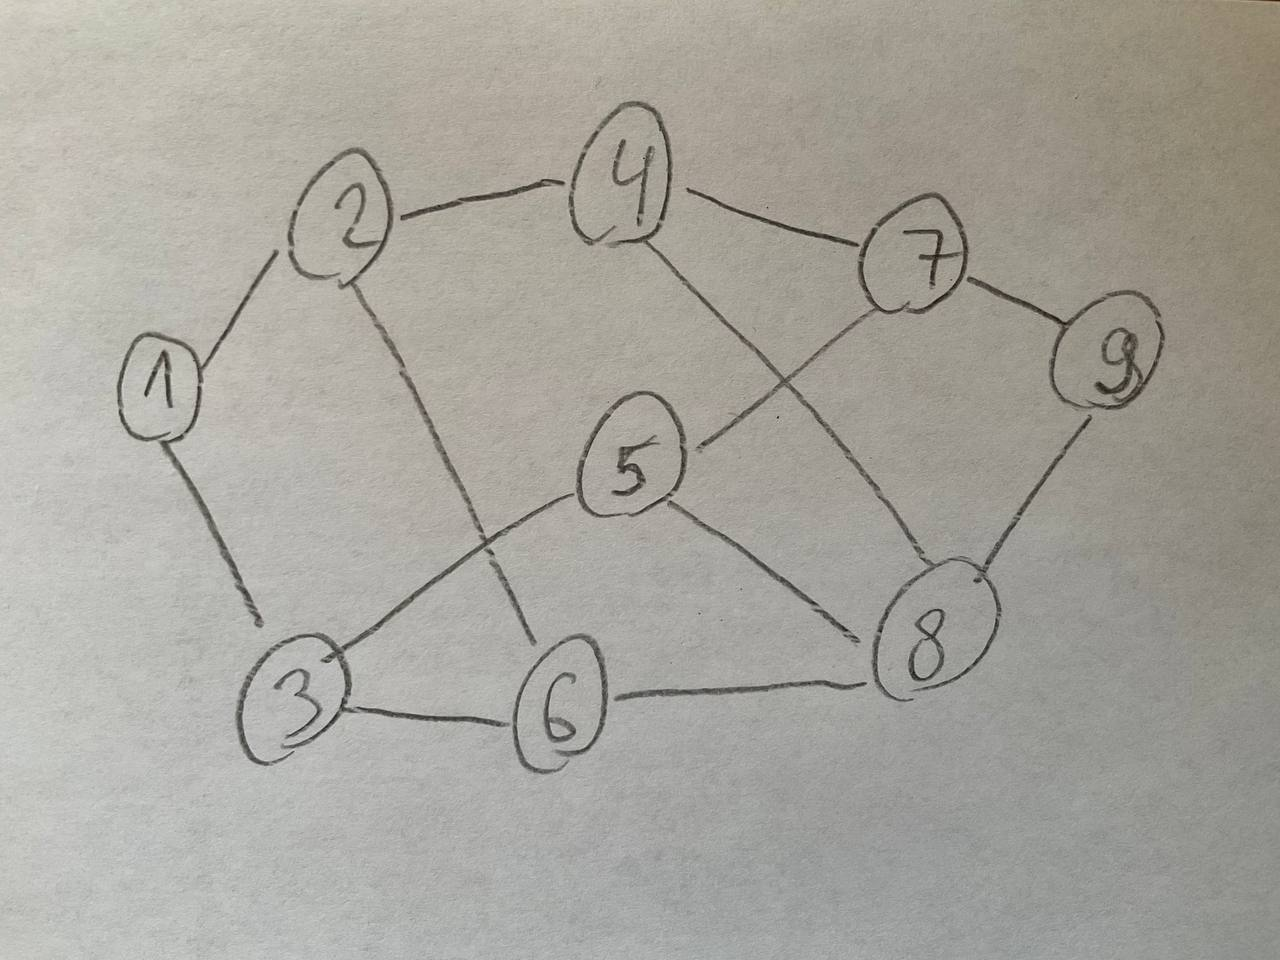
\includegraphics[width=0.8\textwidth]{figures/hand1.jpg}
    \end{figure}
\end{frame}

\begin{frame}{\subsecname}{Mistake}
    \begin{figure}
        \centering
        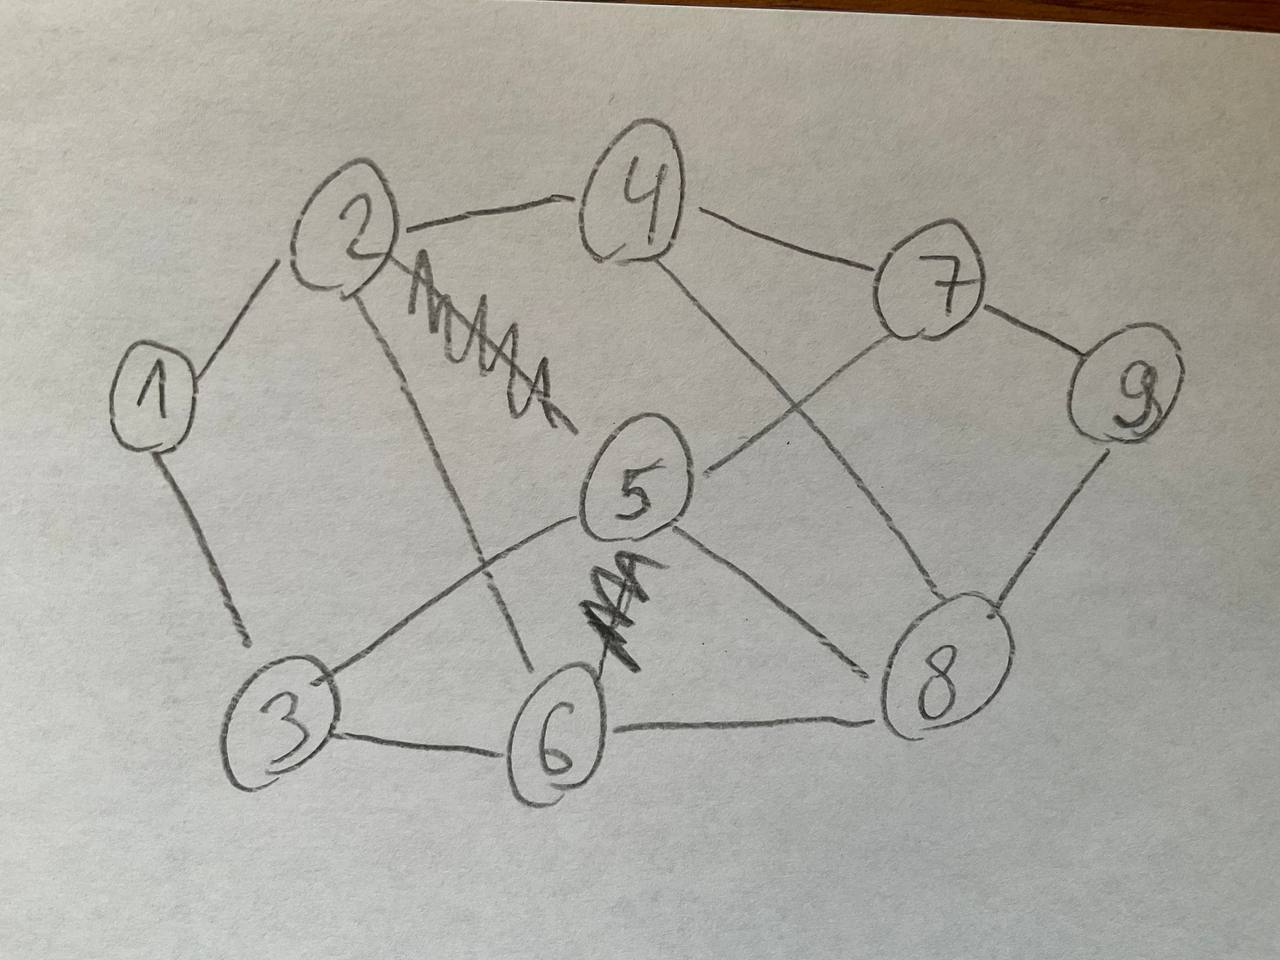
\includegraphics[width=0.8\textwidth]{figures/hand2.jpg}
    \end{figure}
\end{frame}

\begin{frame}{\subsecname}{Mistake}
    \begin{figure}
        \centering
        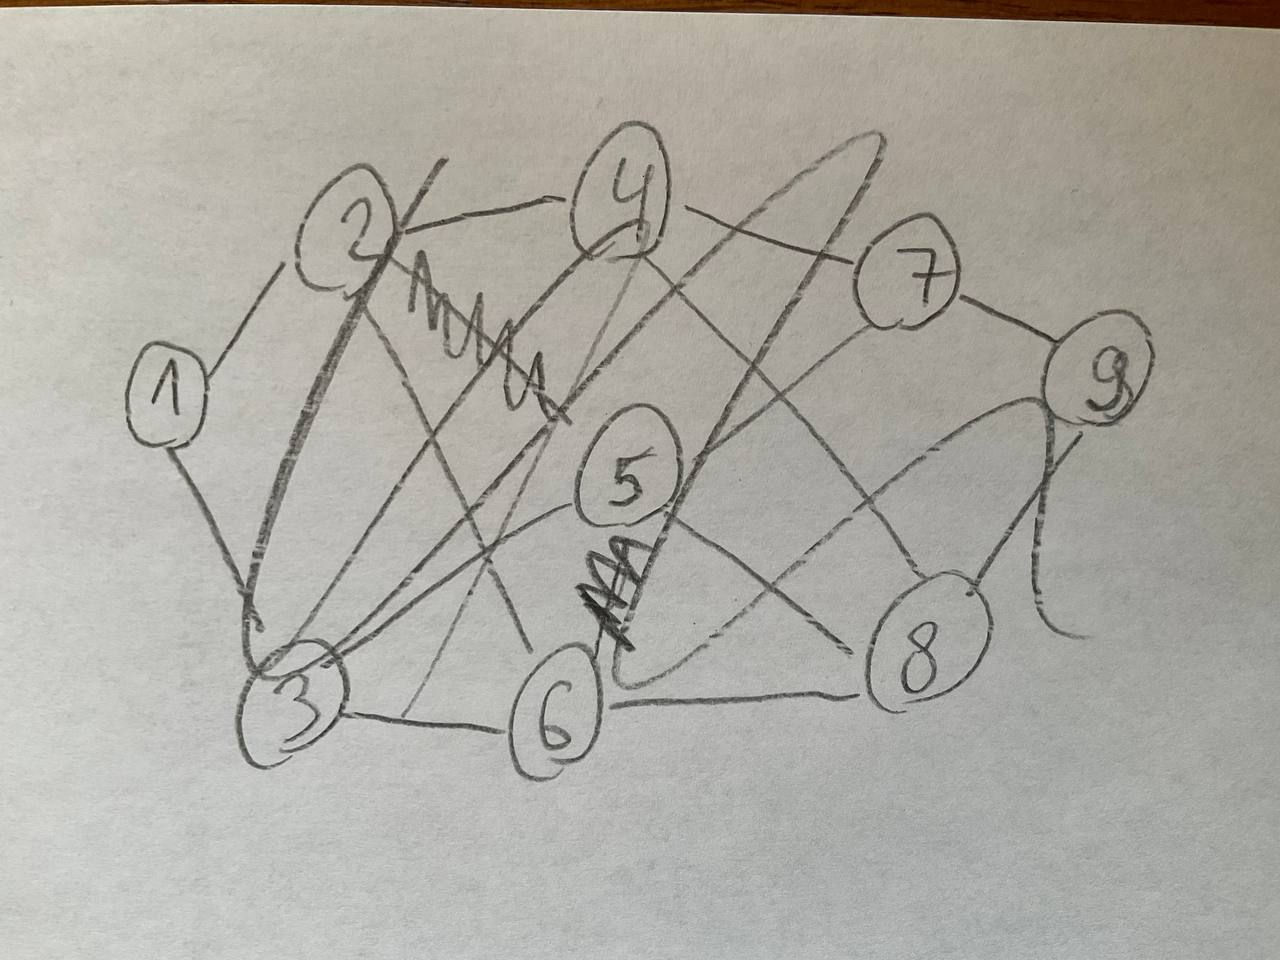
\includegraphics[width=0.8\textwidth]{figures/hand3.jpg}
    \end{figure}
\end{frame}

\subsection{Tablet Drawing}
\begin{frame}{\subsecname}
    \begin{figure}
        \centering
        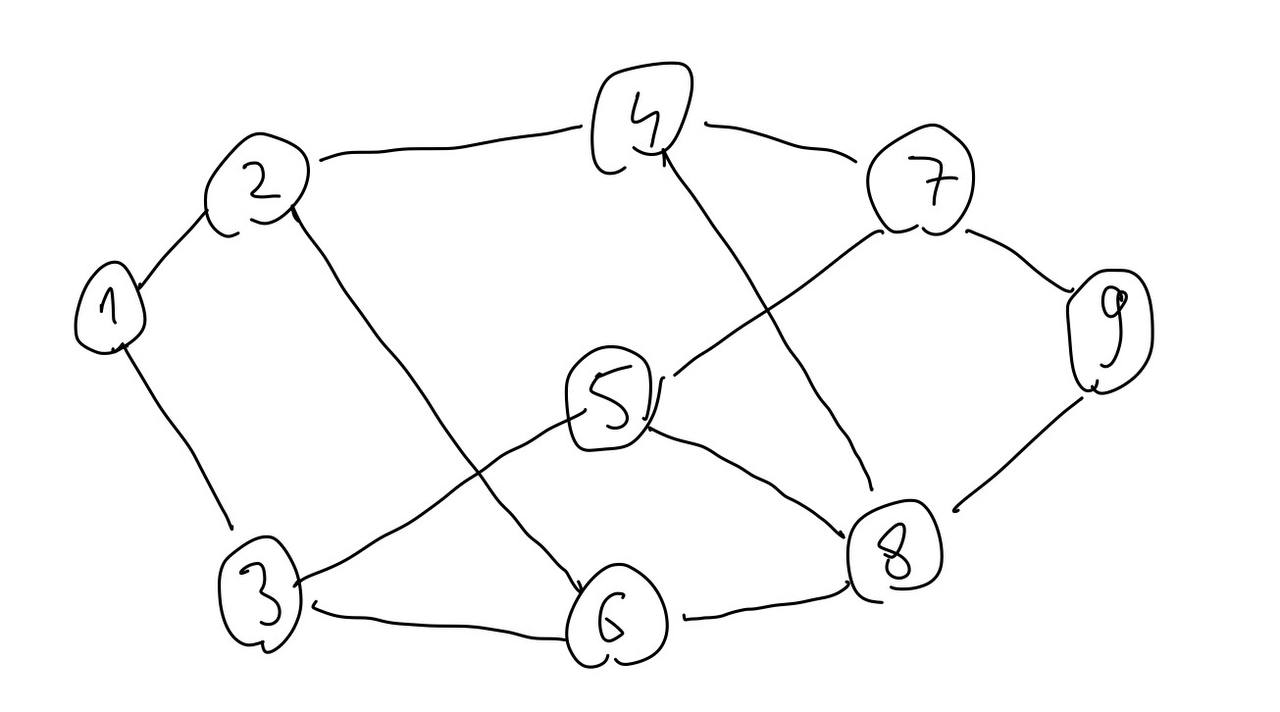
\includegraphics[width=0.8\textwidth]{figures/tablet.jpg}
    \end{figure}
\end{frame}

\subsection{Tikz}
\begin{frame}{\subsecname}
    \begin{figure}[h]
        \centering
        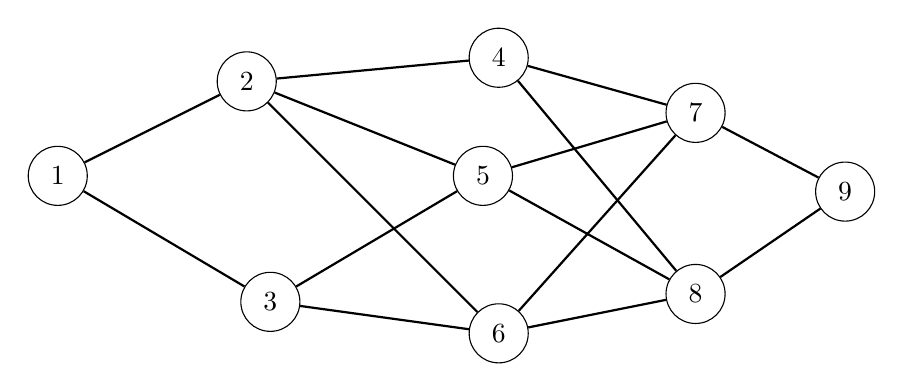
\begin{tikzpicture}[x=10cm,y=10cm]
            \tikzset{     
                e4c node/.style={circle,draw,minimum size=0.75cm,inner sep=0}, 
                e4c edge/.style={sloped,above,font=\footnotesize}
            }
            \node[e4c node] (1) at (0.00, 0.89) {1}; 
            \node[e4c node] (2) at (0.24, 1.01) {2}; 
            \node[e4c node] (3) at (0.27, 0.73) {3}; 
            \node[e4c node] (4) at (0.56, 1.04) {4}; 
            \node[e4c node] (5) at (0.54, 0.89) {5}; 
            \node[e4c node] (8) at (0.81, 0.74) {8}; 
            \node[e4c node] (7) at (0.81, 0.97) {7}; 
            \node[e4c node] (9) at (1.00, 0.87) {9}; 
            \node[e4c node] (6) at (0.56, 0.69) {6}; 
            \path[draw,thick]
                (1) edge[e4c edge]  (2)
                (1) edge[e4c edge]  (3)
                (2) edge[e4c edge]  (4)
                (2) edge[e4c edge]  (5)
                (2) edge[e4c edge]  (6)
                (3) edge[e4c edge]  (5)
                (3) edge[e4c edge]  (6)
                (4) edge[e4c edge]  (7)
                (4) edge[e4c edge]  (8)
                (5) edge[e4c edge]  (7)
                (5) edge[e4c edge]  (8)
                (6) edge[e4c edge]  (7)
                (6) edge[e4c edge]  (8)
                (7) edge[e4c edge]  (9)
                (8) edge[e4c edge]  (9)
                ;
        \end{tikzpicture}
    \end{figure}
\end{frame}

\begin{frame}[fragile]{\subsecname}{Code}
    \begin{block}{}
        \begin{lstlisting}[language=tex]
            \node[e4c node] (1) at (0.00, 0.89) {1}; 
            \node[e4c node] (2) at (0.24, 1.01) {2}; 
            \node[e4c node] (3) at (0.27, 0.73) {3}; 
            \node[e4c node] (4) at (0.56, 1.04) {4}; 
            \node[e4c node] (5) at (0.54, 0.89) {5}; 
            \node[e4c node] (8) at (0.81, 0.74) {8}; 
            \node[e4c node] (7) at (0.81, 0.97) {7}; 
            \node[e4c node] (9) at (1.00, 0.87) {9}; 
            \node[e4c node] (6) at (0.56, 0.69) {6}; 
            \path[draw,thick]
                (1) edge[e4c edge]  (2)
                (1) edge[e4c edge]  (3)
                (2) edge[e4c edge]  (4)
                ...
        \end{lstlisting}
    \end{block}
\end{frame}

\subsection{NetworkX}
\begin{frame}{\subsecname}
\begin{figure}
\resizebox{0.8\textwidth}{!}{\input{figures/fig1.pgf}}
\end{figure}
\end{frame}

\begin{frame}[fragile]{\subsecname}{Code}
    \begin{block}{}
        \begin{lstlisting}[language=python]
G = nx.Graph()
G.add_edges_from([
    (1, 2), (1, 3), (2, 4), (2, 5), (2, 6),
    (3, 5), (3, 6), (4, 7), (4, 8), (5, 7),
    (5, 8), (6, 7), (6, 8), (7, 9), (8, 9)
])
pos = nx.bfs_layout(G, 1)
        \end{lstlisting}
    \end{block}

    \pause

    \begin{block}{Materials for presentation}
        GitHub - \url{https://github.com/Rentib/graph-visualization}
        Google Colab - \url{http://tiny.cc/networkx}
    \end{block}

\end{frame}

\section{How is it done?}
\begin{frame}{\secname}
    \tableofcontents[currentsection,hideothersubsections,sectionstyle=hide]
\end{frame}

\subsection{Overview}
\begin{frame}{\subsecname}
    \begin{block}{Algorithms}
        NetworkX provides several algorithms for graph visualization, focusing
        on different layout strategies to represent nodes and edges effectively.
    \end{block}

    \pause
    \begin{block}{Eye candy}
        \begin{itemize}
            \pause
            \item Nodes, edges, labels, and other graph elements
            \pause
            \item Custom positioning
            \pause
            \item Flexible styling
        \end{itemize}
    \end{block}

    \pause
    \begin{block}{Support}
        \begin{itemize}
            \pause
            \item Image, PDF, SVG, and other formats
            \pause
            \item Interactive visualization using matplotlib
            \pause
            \item \textbf{LaTeX} (Tikz, PGF)
        \end{itemize}
    \end{block}
\end{frame}

\subsection{Bipartite}
\begin{frame}{\subsecname}

    \begin{block}{Algorithm}
        Do 2-coloring and group nodes by color.
    \end{block}

    \pause
    \resizebox{0.8\textwidth}{!}{\input{figures/bipartite.pgf}}
\end{frame}

\subsection{BFS}
\begin{frame}{\subsecname}

    \begin{block}{Algorithm}
        Run breadth first search and group nodes by depth.
    \end{block}

    \pause
    \resizebox{0.8\textwidth}{!}{\input{figures/bfs.pgf}}

\end{frame}

\subsection{ForceAtlas2}
\begin{frame}{\subsecname}
    \begin{block}{Algorithm}
        Out of scope for this presentation, but worth mentioning as the results
        are fantastic.
    \end{block}

    \pause
    \resizebox{0.8\textwidth}{!}{\input{figures/forceatlas2.pgf}}
\end{frame}

\subsection{Force-directed drawings}
\begin{frame}{\subsecname}
    \begin{block}{Analogy to physics}
        \small Edges are \textit{springs}, vertices are \textit{repelling objects}.
    \end{block}
    \pause
    \begin{block}{}
        \scriptsize
        \begin{algorithmic}
            \Function{ForceDirected}{$G = \langle V, E \rangle, p = (p_v)_{v \in V}, \varepsilon > 0, K \in \mathbb{N}$}
                \onslide<3->{\State $l \gets 1$
                \While{$l < K \land \max\limits_{v \in V} \|F_v(t)\| > \varepsilon$}
                    \onslide<4->{
                    \ForAll{$u \in V$}
                        \onslide<5->{\State $F_u(t) \gets \sum\limits_{v \in V} f_{\text{rep}}(u, v) + \sum\limits_{uv \in E} f_{\text{attr}}(u, v)$}
                    \EndFor
                    }
                    \onslide<6->{
                    \ForAll{$u \in V$}
                        \onslide<7->{\State $p_u \gets p_u + \delta(t) \cdot F_u(t)$}
                    \EndFor}
                    \State $l \gets l + 1$
                \EndWhile}
                \State \Return $p$
            \EndFunction
        \end{algorithmic}
    \end{block}
\end{frame}

\section{Conclusion}
\begin{frame}{\secname}
    \begin{block}{}
        NetworkX is \Huge\textcolor{blue}{GREAT!!!}
    \end{block}
\end{frame}

\end{document}
